% Chapter 1

\chapter{Introduction} % Main chapter title

\label{Chapter1} % For referencing the chapter elsewhere, use \ref{Chapter1} 

%----------------------------------------------------------------------------------------

% Define some commands to keep the formatting separated from the content 
\newcommand{\keyword}[1]{\textbf{#1}}
\newcommand{\tabhead}[1]{\textbf{#1}}
\newcommand{\code}[1]{\texttt{#1}}
\newcommand{\file}[1]{\texttt{\bfseries#1}}
\newcommand{\option}[1]{\texttt{\itshape#1}}

%----------------------------------------------------------------------------------------

\section{Dependency Trees}
Dependency trees describe the bilexical relations between pairs of words in a sentence. 
Such relations are drawn from a fixed inventory of grammatical relations~\parencite{jurafsky2000speech}.
For example, Figure \ref{fig:example} shows an example sentence (taken from OntoNotes 5.0~\cite{weischedel2013ontonotes}) with dependency annotations to describe the bilexical relationship between pairs of words. 
\begin{figure}[h!]
	\centering
	\begin{tikzpicture}[node distance=1.0mm and 1.0mm, >=Stealth, 
	wordnode/.style={draw=none, minimum height=5mm, inner sep=0pt},
	chainLine/.style={line width=1pt,-, color=fontgray},
	entbox/.style={draw=black, rounded corners, fill=red!20, dashed}
	]
	\matrix (sent1) [matrix of nodes, nodes in empty cells, execute at empty cell=\node{\strut};]
	{
		They & [1mm]suffer &[1mm]from & [1mm]drug   &  [1mm]  dealing & [1mm]and& [1mm]loitering& [1mm]near & [1mm]their & [1mm]premises\\
	};
	
	\draw [chainLine, ->, color=fontgray, line width=1.5pt] (sent1-1-2) to [out=120,in=60, looseness=1.4] node[above, yshift=-1mm, color=black]{\footnotesize\it nsubj} (sent1-1-1);
	\draw [chainLine, ->] (sent1-1-2) to [out=60,in=120, looseness=1] node[above, yshift=-1mm, color=black]{\footnotesize\it prep} (sent1-1-3);
	\draw [chainLine, ->] (sent1-1-5) to [out=120,in=60, looseness=1] node[above, yshift=-1mm, xshift=-3mm, color=black]{\footnotesize\it prep} (sent1-1-4);
	\draw [chainLine, ->] (sent1-1-3) to [out=60,in=120, looseness=1.4] node[above, yshift=-1mm, color=black]{\footnotesize\it pobj} (sent1-1-5);
	\draw [chainLine, ->] (sent1-1-5) to [out=60,in=120, looseness=1] node[above, yshift=-1mm, color=black, xshift=2mm]{\footnotesize\it cc} (sent1-1-6);
	\draw [chainLine, ->] (sent1-1-5) to [out=60,in=120, looseness=1.5] node[above, yshift=-1mm, color=black, xshift=2mm]{\footnotesize\it conj} (sent1-1-7);
	\draw [chainLine, ->] (sent1-1-5) to [out=60,in=120, looseness=1.5] node[above, yshift=-1mm, color=black]{\footnotesize\it prep} (sent1-1-8);
	\draw [chainLine, ->, color=fontgray, line width=1pt] (sent1-1-10) to [out=120,in=60, looseness=1.4] node[above, yshift=-1mm, color=black, xshift=-3mm]{\footnotesize\it poss} (sent1-1-9);
	\draw [chainLine, ->, line width=1pt] (sent1-1-8) to [out=60,in=120, looseness=1.5] node[above, yshift=-1mm]{\footnotesize\textit{\textbf{pobj}} } (sent1-1-10);		
	\end{tikzpicture} 
	\caption{Example sentences annotated with dependency structures.}
	\label{fig:example}
\end{figure}

The word ``\textit{They}'' is the subject of the verb ``\textit{suffer}'', and ``\textit{from}'' is the preposition of this verb. 
Overall, we can see that each word has exactly one parent as in the dependency trees except for the root (i.e., ``\textit{suffer}'' in this case).
On the other hand, this tree is \textbf{\textit{projective}} in the sense that there is no crossing edge in the dependency trees. 
According to \citet{jurafsky2000speech}, an arc from a head to a dependent is said to be projective if there is a path from the head to every word that lies between the head and the dependent in the sentence. 
A dependency tree is then said to be projective if all the arcs that make it up are projective. 
Most of the dependency trees in English are projective while non-projective dependencies are also allowed, particularly for some languages with flexible word orders, such as Czech.

As different languages have different forms of dependencies as well as different types of dependency relations, \textit{Universal Dependencies}\footnote{https://universaldependencies.org/}~\cite{nivre2016universal} are proposed to consistently unify the grammar across different languages.
%As of today, there are 157 treebanks for 90 languages. 
The speedy progress of universal dependencies allows us to work on the downstream tasks by making use of such dependency trees. 


%----------------------------------------------------------------------------------------

\section{Motivation}



%%% rough motivation
Motivated by the fact that the dependency trees convey semantic-level information, we focus on the structured prediction tasks of named entity recognition~\cite{tjong2003introduction} and semantic parsing which requires a semantic-level understanding of natural languages. 
Specifically, we study the underlying connections between the dependency trees and the output structures (\textit{e.g.}, named entity sequences and structured meaning representation) based on our observation from existing datasets. 
We raise several research questions in this thesis for us to exploit the connections for the downstream tasks. 


\subsection{Dependency-Guided Named Entity Recognition}
Though the dependencies describe the bilexical relations between pairs of words, we should be aware that some words that form a named entity should be treated as a \textit{complete} unit in the dependency trees. 
For example, the \textsc{gpe} entity ``\textit{Hong Kong}'' is a complete unit and it should form a subtree in the following example. 
The same applies to the \textsc{event} entity ``\textit{seminar on the actual practice of tax reform}''. 

\begin{figure}[h!]
	\centering
	%	\includegraphics[width=2.8in]{imgs/example.pdf}
	\adjustbox{max width=1.0\linewidth}{
		\begin{tikzpicture}[node distance=1.0mm and 1.0mm, >=Stealth, 
		wordnode/.style={draw=none, minimum height=5mm, inner sep=0pt},
		chainLine/.style={line width=1pt,-, color=fontgray},
		entbox/.style={draw=black, rounded corners, fill=red!20, dashed}
		]
	
		
		
		\matrix (sent2) [matrix of nodes, nodes in empty cells, execute at empty cell=\node{\strut};]
		{
			The &[-1mm] seminar &[-1mm] on &[-1mm] the & [-1mm]actual   &    [-1mm]practice &[-1mm] of & [-1mm]tax& [-1mm]reform & [-1mm]was & [-1mm]held & [-1mm]in &[-1mm] Hong &[-1mm] Kong\\
			%		 \textbf{\textsc{date}}   &   &   & \textsc{o}     & \textsc{o}   & \textsc{o}  & \textsc{o}& \textsc{event} &  \\
		};
		
		\draw [chainLine, ->] (sent2-1-2) to [out=120,in=60, looseness=1] node[above, yshift=-1mm, xshift=0mm,  color=black]{\footnotesize\it det} (sent2-1-1);
		\draw [chainLine, <-] (sent2-1-3) to [out=120,in=60, looseness=1.5] node[above, yshift=-1.5mm,  color=black, xshift=2mm]{\footnotesize\it prep} (sent2-1-2);
		\draw [chainLine, ->] (sent2-1-6) to [out=120,in=60, looseness=1.5] node[above, yshift=-1mm, xshift=-1mm,  color=black]{\footnotesize\it det} (sent2-1-4);
		\draw [chainLine, ->] (sent2-1-6) to [out=120,in=60, looseness=1] node[above, yshift=-1mm, xshift=-2mm,  color=black]{\footnotesize\it amod} (sent2-1-5);
		\draw [chainLine, ->] (sent2-1-3) to [out=60,in=120, looseness=1.6] node[above, yshift=-1.5mm,  color=black]{\footnotesize\it pobj} (sent2-1-6);
		\draw [chainLine, ->] (sent2-1-6) to [out=60,in=120, looseness=1.5] node[above, yshift=-1.5mm,  color=black]{\footnotesize\it prep} (sent2-1-7);
		\draw [chainLine,<-, line width=1pt] (sent2-1-8) to [out=60,in=120, looseness=1.5] node[above, yshift=-1mm, color=black,xshift=-1mm]{\footnotesize\it nn} (sent2-1-9);
		\draw [chainLine, ->] (sent2-1-7) to [out=60,in=120, looseness=1.8] node[above, yshift=-1.5mm,  color=black]{\footnotesize\it pobj} (sent2-1-9);
		
		\draw [chainLine,->, line width=1pt] (sent2-1-9) to [out=60,in=120, looseness=1.5] node[above, yshift=-1mm, color=black,xshift=-1mm]{\footnotesize\it auxpass} (sent2-1-10);
		\draw [chainLine, ->] (sent2-1-11) to [out=60,in=120, looseness=3.0] node[above, yshift=-1.5mm,  color=black]{\footnotesize\it prep} (sent2-1-12);
		
		\draw [chainLine, ->, color=fontgray, line width=1pt] (sent2-1-12) to [out=60,in=120, looseness=1.6] node[above, yshift=-1.5mm,  color=fontgray]{\footnotesize\it pobj} (sent2-1-14);
		\draw [chainLine, <-] (sent2-1-13) to [out=60,in=120, looseness=1.4] node[above, yshift=-1mm,  color=black, xshift=-1mm]{\footnotesize\it nn} (sent2-1-14);
		
		\draw [chainLine, <-, color=fontgray, line width=1pt] (sent2-1-2) to [out=60,in=120, looseness=0.8] node[above, yshift=-1mm,  color=fontgray, xshift=-1mm]{\footnotesize\it nsubjpass} (sent2-1-11);
		
		
		\begin{pgfonlayer}{background}
		\node [entbox, below=of sent2-1-5, xshift=5.7mm, yshift=5.8mm, text height=8mm, minimum width=78mm, fill=myblue!20] (e2)  [] {\color{blue!80}\textbf{\textsc{event}}};
		\node [entbox, below=of sent2-1-13, xshift=5mm, yshift=6.5mm, text height=8mm, minimum width=20mm, fill=yellow!40] (e2)  [] {\color{blue!80}\textbf{\textsc{gpe}}};
		\end{pgfonlayer}
		\end{tikzpicture} 
	}
	%	\vspace*{-7.5mm}
	\caption{Example sentences annotated with named entities and dependencies in the OntoNotes 5.0 dataset.}
	%	\vspace*{-6mm}
	\label{fig:examples}
\end{figure}

By observing the named entity datasets with dependency annotations, we found that most of the entities often form dependency subtrees in a sentence~\cite{jie2017efficient}. 
On the other hand, certain entities have strong correlations with the dependency relations~\cite{jie2019dependency}. 
For example, in the OntoNotes dataset~\cite{weischedel2013ontonotes}, 61\% of \textsc{norp} (i.e., Nationalities or religious or political groups) entities attach to the dependency relations \textit{amod} (i.e., adjectival modifier). 

The major research challenge is how we can make use of these two types of relationships to improve our named entity recognition systems. 
We ask the following three research questions: 
\begin{itemize}
	\item \textit{We know entities form subtrees in the dependencies. Can we impose certain constraints in the NER models to filter out some candidates that cannot form subtrees?}
	\item \textit{Besides, how to incorporate the complete structured information provided by the dependency trees for NER?}
	\item \textit{What if we do not have the complete annotations for NER? How does the dependency help in such a scenario?}
\end{itemize}

We aim to design efficient models to solve these two research questions and capture the complete structured information in our model architecture~\cite{jie2017efficient,jie2019dependency}. 
The third question is an actual incomplete annotation scenario~\cite{jie2019better} and the relationship between the dependency and named entities may take a role in such a scenario. 

\subsection{Dependencies in Semantic Parsing}
Semantic parsing is a fundamental task within the field of natural language processing (NLP).
Semantic parsing aims to transform the natural language sentences into machine-interpretable meaning representations automatically. 
On the other hand, the previous work~\cite{reddy2016transforming} shows that dependency trees leverage shallow semantic information. 

\begin{figure}[h!]
	\centering
	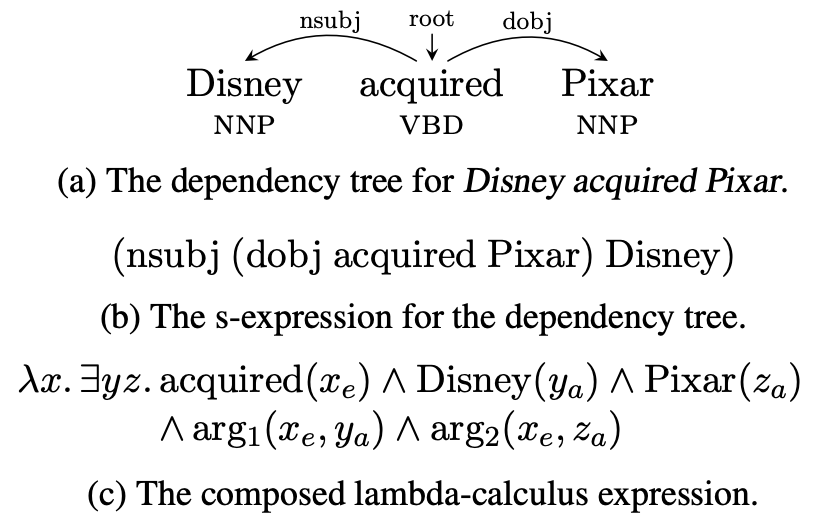
\includegraphics[width=4in]{Figures/dep2lambda.png}
	\caption{Example of transforming dependency into logical forms (taken from \citet{reddy2016transforming}).}
	\label{fig:transformexample}
\end{figure}

The underlying observation is helpful for extracting semantic meaning representation from the dependency trees. 
\citet{reddy2016transforming,reddy2017universal} proposed a supervised learning approach to transform the universal dependencies into lambda-calculus expression. 
Similarly, \citet{wang2015transition} proposed a transition-based algorithm to convert the dependency trees into abstract meaning representations (AMR).
Universal dependencies are obtained by training the dependency parsers using the Universal dependency treebanks.
They demonstrated the new state-of-the-art semantic parsing results on certain datasets. 
%On the other hand, dependency trees which leverage shallow semantic information are helpful for semantic parsing~\cite{reddy2016transforming}. 
%\citet{reddy2016transforming} transforms the preprocessed dependency tree structures into lambda-calculus expression. 
However, their semantic parsing performance largely depends on the quality of the dependency parsers. 
Without enough training data, it is not guaranteed that we can have a high-quality dependency parser. 
Thus, we raise the following research question:
\begin{itemize}
	\item \textit{Can we extract the dependency tree without the dependency annotations in the semantic parsing task?}
\end{itemize}
Our goal here is to design a structured model that regards the dependency tree as a latent variable in the semantic parsing task. 
%Our further attempt is to 
%dependency tree annotations are often not available in the datasets for semantic parsing. 
%How to extract such a dependency tree structure remains a research challenge in the semantic parsing task. 

%----------------------------------------------------------------------------------------

\section{Thesis Outline}


The thesis is organized as follows:
\begin{itemize}
	\item Chapter \ref{Chapter2} presents the background of named entity recognition and semantic parsing. 
	We introduce the task definitions, the current approaches and the challenges in these structured prediction tasks.
%	introduces the relevant literature on applying syntactic dependency trees for semantic-level structured prediction tasks, especially NER and semantic parsing. 
	
	\item Chapter \ref{Chapter3} presents the structured relationships between the dependency trees and semantically meaningful named entities. 
	We propose our dependency-guided model based on the semi-Markov conditional random fields (semi-CRF) and conduct experiments on several datasets.
	The experimental results demonstrate that our model is much more efficient than the semi-CRF and achieves comparable or even better performance than the semi-CRF model.
%	We further demonstrate that such relationships are able to significantly improve the performance of NER, especially for the European languages. 
	
	\item Chapter \ref{Chapter4} further shows deeper relationships between the dependency trees and named entities, including the long-distance interactions and correlations between the dependency relations and the named entity types. 
	In order to fully exploiting these relationships, we  propose a dependency-guided LSTM CRF model to capture these properties. 
	Our large-scale experiments on the datasets with four languages demonstrate the proposed model is effective across different languages and the dependencies are consistently helpful.
	
	
	\item Chapter \ref{Chapter5} presents a practical scenario of incomplete annotations in NER.
	Specifically, we do not assume \textsc{o} labels are available in incomplete annotations. 
	We propose the iterative training solution and discuss the inefficiency of this approach. 
	However, such an iterative approach is not efficient during training. 
	In order to address the inefficiency, we further present the dependency-based solution to this problem as our future work. 
	
	\item Chapter \ref{Chapter6} further studies the semantics leveraged from the dependency trees. 
	We build the connections between the dependency trees and the meaning representations in semantics. 
	We then present a dependency-based hybrid tree representation to capture the interaction between the natural language and the tree-structured meaning representation. 
	We discuss the expressiveness of such a  hybrid tree representation.  
	Such hybrid trees are latent and can be learned by a structured latent-variable model. 
	We also present a potential dependency hybrid tree solution to recently popular meaning representation, SQL.
	
	
	\item Chapter \ref{Chapter7} presents the potential research directions besides the contribution in this thesis, such as joint dependency parsing and named entity recognition.
%	presents some research challenges regarding the requirement of dependency.
	We also argue that the linear-chain model might not always be the best fit for any languages and propose some future directions in better design of a universal named entity recognition system in terms of different languages.
	We  also point out some future research directions for universal semantic parsing using one framework for different types of meaning representations. 
	
	\item Chapter \ref{Chapter8} concludes the strong connections between the dependency trees and semantic representation
	 in natural language as well as how dependencies benefit the language understanding.
	We summarize the overall research contribution in this thesis and what we would like to do in the future.
\end{itemize}


\section{Contributions}

Our overall contributions throughout the PhD study can be summarized as follows:
\begin{itemize}
	\item Statistically, we found the strong structured relationship between the dependency trees and named entities. 
	Such a relationship leverages the named entities often form subtrees in the dependency trees and attach to certain specific dependency relations. 
	\item Through the observation, we are able to make use of this property to build efficient dependency-guided models for named entity recognition (NER). 
	Motivated by the structured relationship, we can reduce the search space for an NER model~\cite{jie2017efficient} to have efficient inference speed.  
	We developed an efficient dependency-guided model (DGM) based on the semi-Markov CRF. 
	Such a DGM model enjoys the linear-time average complexity while having comparable performance as the semi-Markov CRF which has $L$-times larger complexity. 
	\item On the other hand, such a relationship allows us to design a better dependency-guided neural architecture~\cite{jie2019dependency} rather than simply bidirectional long short-term memory (BiLSTM) networks~\cite{hochreiter1997long}.
	We demonstrate that our dependency-guided neural architecture is able to improve the NER performance by capturing the above relationship between the named entities and dependencies on the datasets with several languages. 
	\item We introduce a practical scenario of named entity recognition with incomplete annotations~\cite{jie2019better} and propose an iterative training solution to this problem. 
	Our scenario does not assume \textsc{o} labels are always available in practice and the proposed approach iteratively recovers the \textsc{o} labels.
	Though this solution achieves state-of-the-art performance in such a scenario, the training time is extremely expensive. 
	To find an efficient solution, we further discuss a dependency-based approach by applying the relationships presented in the above sections as our future work. 
	\item We further explore the deeper relationship between the dependency trees and semantic representations. 
	Though the previous work~\cite{reddy2016transforming} has been working on transforming the dependency trees (with shallow semantics) into meaning representation, we focus on extracting the meaningful dependency trees without explicit dependency tree annotations~\cite{jie2018dependency}. 
	We present a novel {\em dependency-based hybrid tree} representation that captures both words and semantics in a joint manner.
	As a result, such a dependency-based hybrid tree largely benefits the task of semantic parsing, especially for languages with flexible word order.
	
%	\item Finally, we 
%	\item We present a novel model that is able to explicitly exploit the global structured information conveyed by dependency trees, showing that such information can be effectively integrated into the process of performing NER. To the best of our knowledge, this is the first  work that exploits such information for NER.
%	\item Theoretically, we show through average-case time complexity analysis that our model has the same time complexity as that of the linear-chain CRFs, and is better than that of the semi-Markov CRFs.
%	\item Empirically, we demonstrate the benefits of our approach through extensive experiments on benchmark datasets.
%	We show that the resulting  model leads to NER results that are competitive with the baseline approach based on semi-Markov CRFs, while requiring significantly less running time.
%	\item We present a novel {\em dependency-based hybrid tree} representation that captures both words and semantics in a joint manner.
%	Such a dependency tree reveals semantic dependencies between words which are easily interpretable. 
%	
%	%	\item We build a semantic parser with such a representation, presenting 
%	\item We show that exact dynamic programming algorithms for inference can be designed on top of our new representation.  We further show that the model can be integrated with neural networks for improved effectiveness.
%	%	propose a neural graphical model to learn the latent {\em dependency-based hybrid tree} structure. 
%	%		Our efficient dynamic-programming algorithm allows the model to perform tractable inference over the graphical model and the neural networks. 
%	\item Extensive experiments conducted on the standard multilingual GeoQuery dataset 
%	%	with eight languages
%	show that our model outperforms the state-of-the-art models on 7 out of 8 languages. Further analysis confirms the effectiveness of our  dependency-based representation.
\end{itemize}

